
\documentclass[paper=a4, fontsize=11pt]{scrartcl} % A4 paper and 11pt font size

\usepackage[T1]{fontenc} % Use 8-bit encoding that has 256 glyphs
\usepackage{fourier} % Use the Adobe Utopia font for the document - comment this line to return to the LaTeX default
\usepackage[english]{babel} % English language/hyphenation
\usepackage{amsmath,amsfonts,amsthm} % Math packages
\usepackage{tabularx}
\usepackage{outlines}
\usepackage{framed,varwidth}
\usepackage{enumitem}
\usepackage{lipsum} % Used for inserting dummy 'Lorem ipsum' text into the template
\usepackage[left=0.5in, right=0.5in, top=3in, bottom=.25in]{geometry}
\geometry{}
\usepackage{sectsty} % Allows customizing section commands
\usepackage{graphicx}
\usepackage{fancyhdr} % Custom headers and footers
\usepackage{listings}
\usepackage{color}


\sectionfont{\centering \normalfont\scshape} % Make all sections centered, the default font and small caps
\pagestyle{fancyplain} % Makes all pages in the document conform to the custom headers and footers
\fancyhead{} % No page header - if you want one, create it in the same way as the footers below
\fancyfoot[L]{} % Empty left footer
\fancyfoot[C]{} % Empty center footer
\fancyfoot[R]{\thepage} % Page numbering for right footer
\renewcommand{\headrulewidth}{0pt} % Remove header underlines
\renewcommand{\footrulewidth}{0pt} % Remove footer underlines
\setlength{\headheight}{0pt} % Customize the height of the header

\numberwithin{equation}{section} % Number equations within sections (i.e. 1.1, 1.2, 2.1, 2.2 instead of 1, 2, 3, 4)
\numberwithin{figure}{section} % Number figures within sections (i.e. 1.1, 1.2, 2.1, 2.2 instead of 1, 2, 3, 4)
\numberwithin{table}{section} % Number tables within sections (i.e. 1.1, 1.2, 2.1, 2.2 instead of 1, 2, 3, 4)

\graphicspath{{./}}
%\setlength\parindent{0pt} % Removes all indentation from paragraphs - comment this line for an assignment with lots of text

\makeatletter
	\newcommand*\variableheghtrulefill[1][.4\p@]
	{%
		\leavevmode
		\leaders \hrule \@height #1\relax \hfill
		\null
	}
\makeatother


%----------------------------------------------------------------------------------------
%	TITLE SECTION
%----------------------------------------------------------------------------------------

\newcommand{\horrule}[1]{\rule{\linewidth}{#1}} % Create horizontal rule command with 1 argument of height
% \title{Template: Homework 1}
\title{	
\normalfont \normalsize 
%\textsc{Rutgers University, Real Analysis I} \\ [25pt] % Your university, school and/or department name(s)
\horrule{0.5pt} \\[0.4cm] % Thin top horizontal rule
\huge CMPSC 360: Homework 01 \\ % The assignment title
\horrule{2pt} \\[0.5cm] % Thick bottom horizontal rule
}

\author{\textbf{\underline{Name:}}Kyle Salitrik | \textit{\textbf{\underline{ID\#:}} 997543474} | \textit{\textbf{\underline{PSU ID:}} kps168}} % Your name

\date{\normalsize\today} % Today's date or a custom date

\begin{document}

\maketitle % Print the title

%----------------------------------------------------------------------------------------
%	PROBLEM 1
%----------------------------------------------------------------------------------------
\newgeometry{top=.75in, bottom=.75in, left=1.25in,right=1.25in}
\section*{\variableheghtrulefill[.25ex]\quad Problem 1 \quad\variableheghtrulefill[.25ex]}

\begin{center}
  \fbox{\quad%
    \begin{varwidth}{\linewidth}
    	Given $|A| = n \implies |P(A)| = 2^n$, demonstrate the power set for: $P(A) = {7,4,5,0,9}$
    \end{varwidth}%
  \quad}
\end{center}

Since $|A| = 5$, we know that $|P(A)| = 2^5$, therefore $P(A)$ has 32 subsets.
\begin{align*}
	P = & (\{\}, \{7\},\{4\},\{7,4\}, \{5\},\{7,5\},\{4,5\}, \{7, 4, 5\}, \{0\},\{7,0\}, \{4, 0\}, \{7, 4, 0\},\{5,0\},\{7,5,0\}, \{4, 5, 0\}, \{7, 4, 5, 0\}, \\
	&\{9\},\{7,9\},\{4,9\}, \{7, 4, 9\}, \{5,9\},\{7,5,9\}, \{4,5,9\}, \{7, 4, 5, 9\}, \{0, 9\},\{7,0,9\},\{4,0,9\}, \{7, 4, 0,9\}, \{5, 0, 9\}, \\
	& \{7, 5, 0, 9\}, \{4, 5, 0, 9\},\{7, 4, 5, 0, 9\})
\end{align*}


%----------------------------------------------------------------------------------------
%	PROBLEM 2
%----------------------------------------------------------------------------------------
\section*{\variableheghtrulefill[.25ex]\quad Problem 2 \quad\variableheghtrulefill[.25ex]}

\begin{center}
  \fbox{\quad%
    \begin{varwidth}{\linewidth}
    	Check if the expression $[\neg (P \iff Q) \land R] \iff [\neg R \lor ((P \lor Q) \lor (P \land Q))]$
    	\begin{enumerate}[label=(\alph*)]
    		\item is a tautology, contradiction or contingency.
    		\item Make a truth table for this set.
    		\item Make the Venn diagram representation.
    		\item Make the logic circuit gate representation.
    		\item Make the code representation.
    	\end{enumerate}
    \end{varwidth}%
  \quad}
\end{center}

\subsection*{a)}
\quad The expression is a contingency and simplifies to $R \land (\neg P \lor \neg Q)$.
\subsection*{b)}
	\makebox[\textwidth][c]{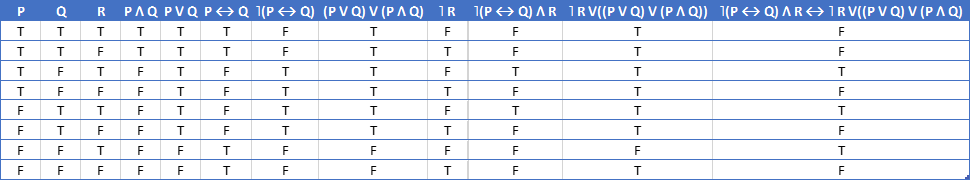
\includegraphics[width=.9\pagewidth]{p2-table}}
\subsection*{c)}
	\makebox[\textwidth][c]{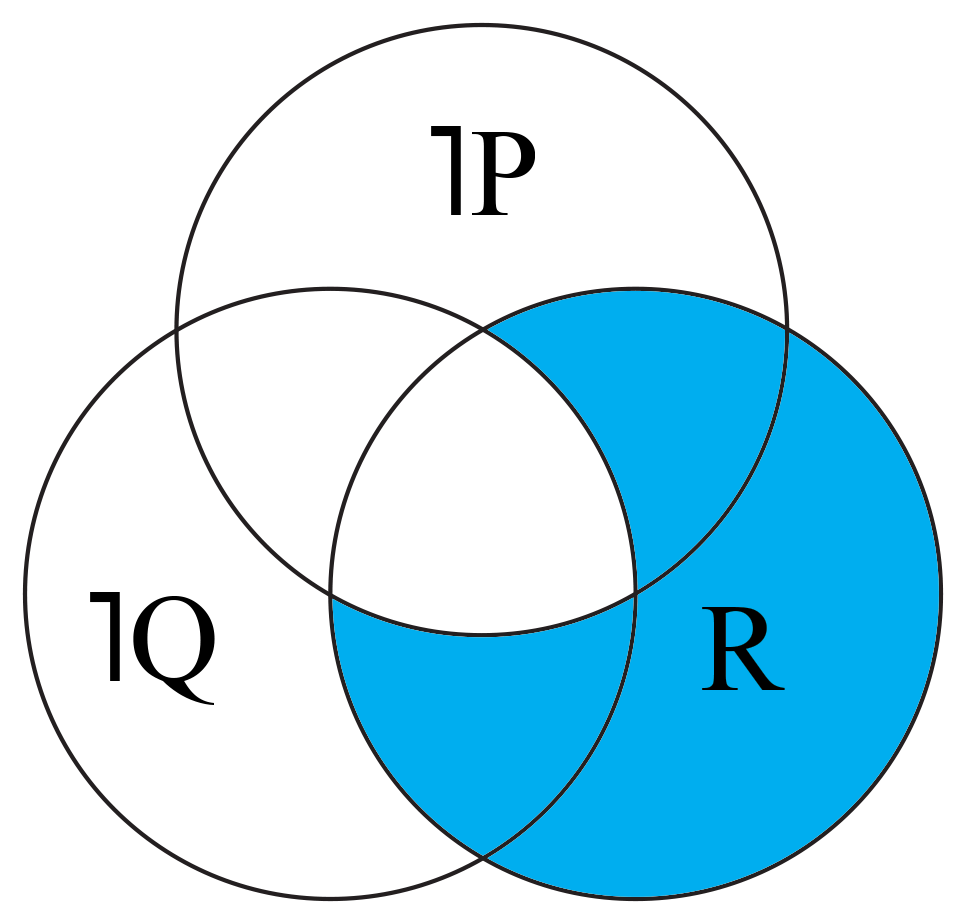
\includegraphics[width=.3\pagewidth]{p2-venn}}
\subsection*{d)}
	\makebox[\textwidth][c]{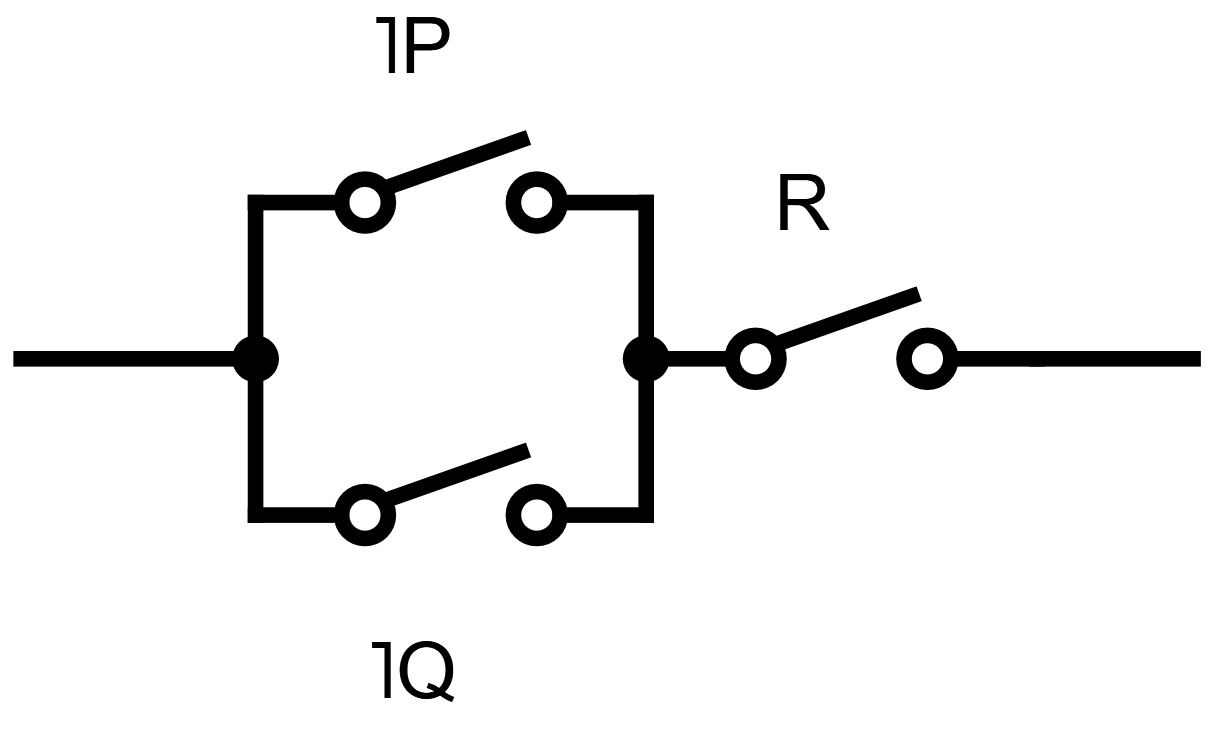
\includegraphics[width=.4\pagewidth]{p2-circuit}}
%	\newgeometry{top=.75in, bottom=.75in, left=.25in,right=.25in}
\subsection*{e)}
	\lstset
	{
		language=C++,
%		basicstyle=\ttfamily,
%		keywordstyle=\color{blue}\ttfamily,
%		stringstyle=\color{red}\ttfamily,
%		commentstyle=\color{green}\ttfamily,
%		morecomment=[l][\color{magenta}]{\#}
		keywordstyle=\color{blue},
		stringstyle=\color{red},
		commentstyle=\color{green},
		morecomment=[l][\color{magenta}]{\#}
	}
	\lstinputlisting[firstline=4]{CMPSC360_Homework.cpp}

%	\newgeometry{top=.75in, bottom=.75in, left=1.25in,right=1.25in}

%----------------------------------------------------------------------------------------
%	PROBLEM 3
%----------------------------------------------------------------------------------------
\section*{\variableheghtrulefill[.25ex]\quad Problem 3 \quad\variableheghtrulefill[.25ex]}

\begin{center}
  \fbox{\quad%
    \begin{varwidth}{\linewidth}
		\textbf{\underline{Simplify:}} \\
		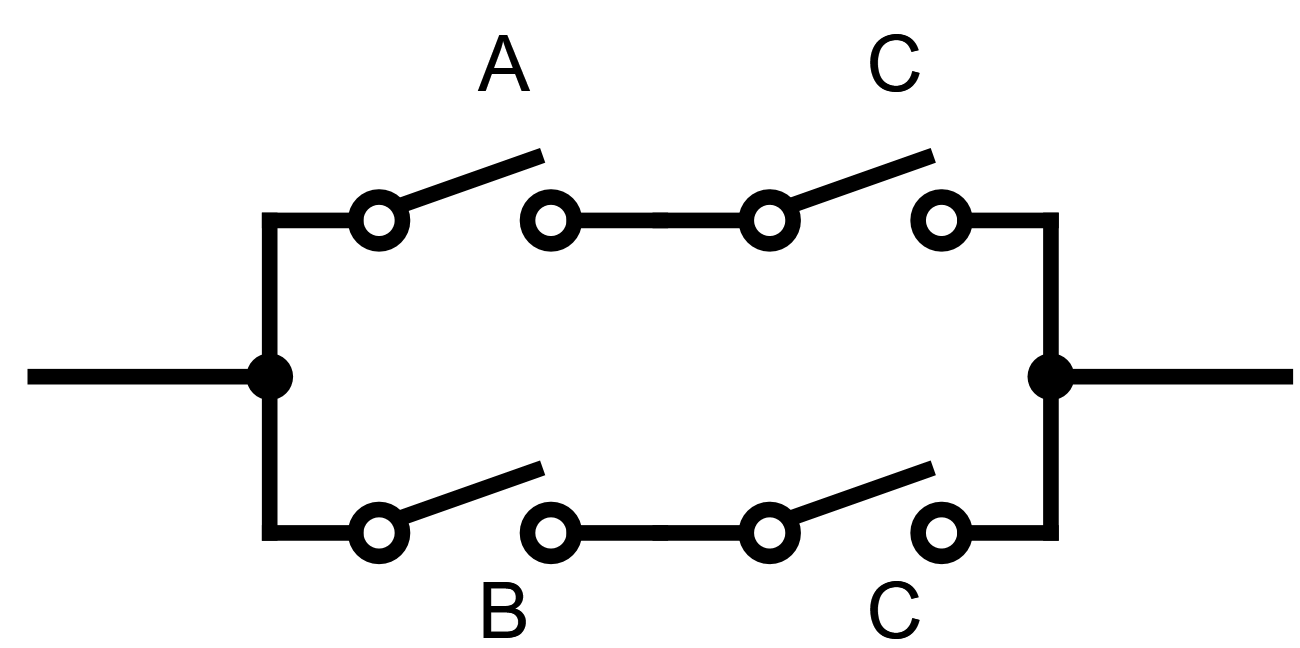
\includegraphics[scale=1.5]{problem3}
    \end{varwidth}
  \quad}
\end{center}

\makebox[\textwidth][c]{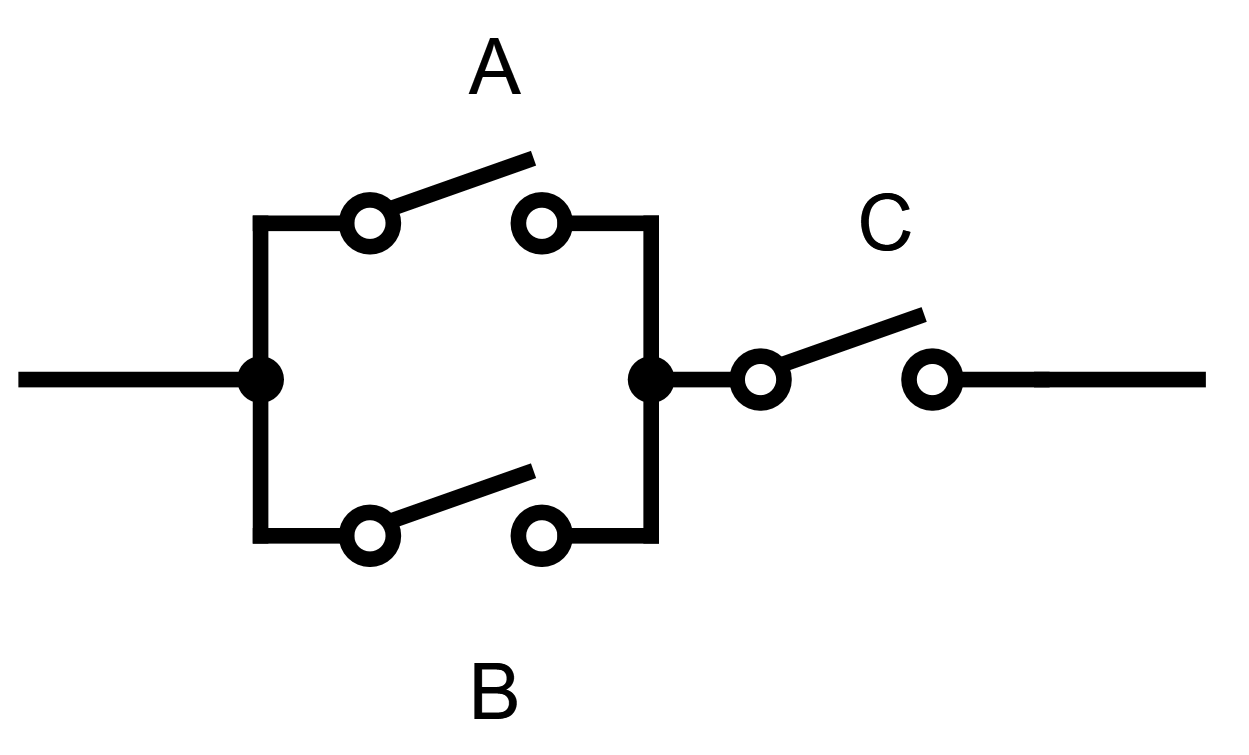
\includegraphics[width=.25\pagewidth]{p3-circuit}}


%----------------------------------------------------------------------------------------
%	PROBLEM 4
%----------------------------------------------------------------------------------------
\section*{\variableheghtrulefill[.25ex]\quad Problem 4 \quad\variableheghtrulefill[.25ex]}

\begin{center}
  \fbox{\quad%
    \begin{varwidth}{\linewidth}
		\textbf{\underline{Simplify:}} \\
		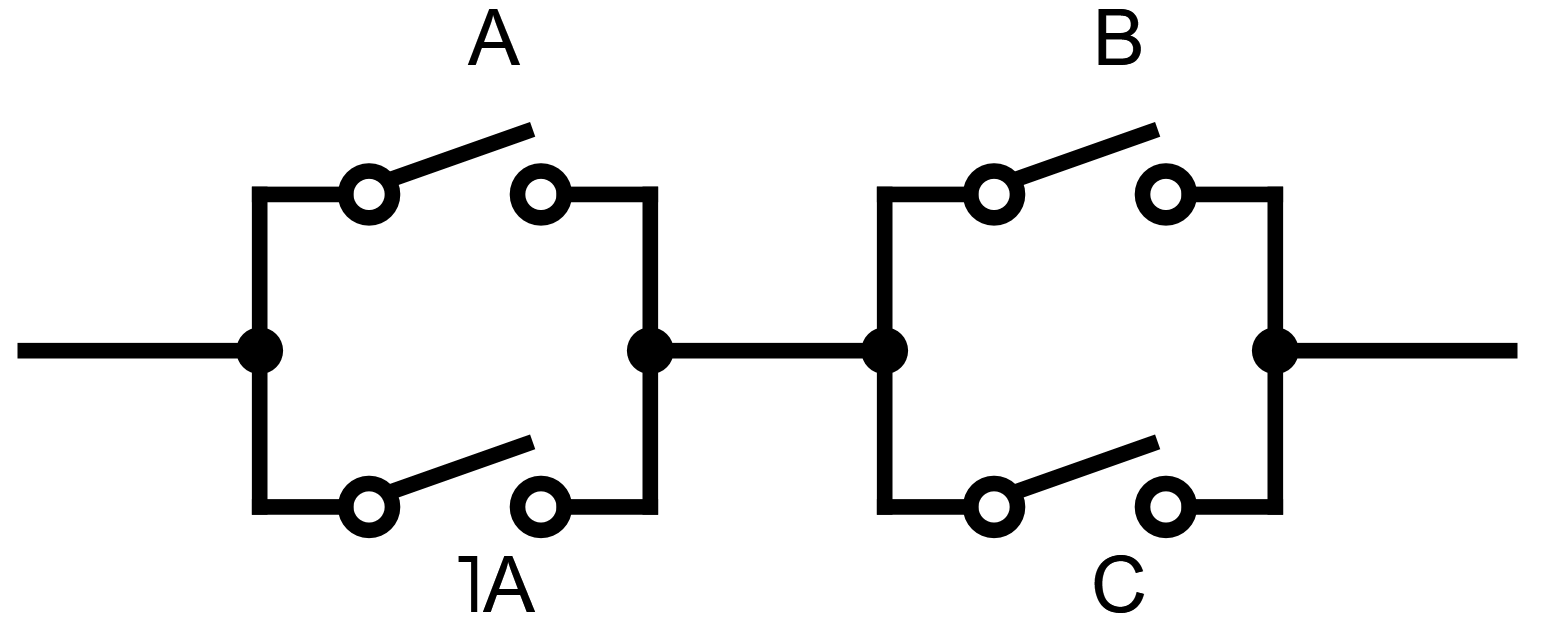
\includegraphics[scale=1.5]{problem4}
    \end{varwidth}%
  \quad}
\end{center}

\makebox[\textwidth][c]{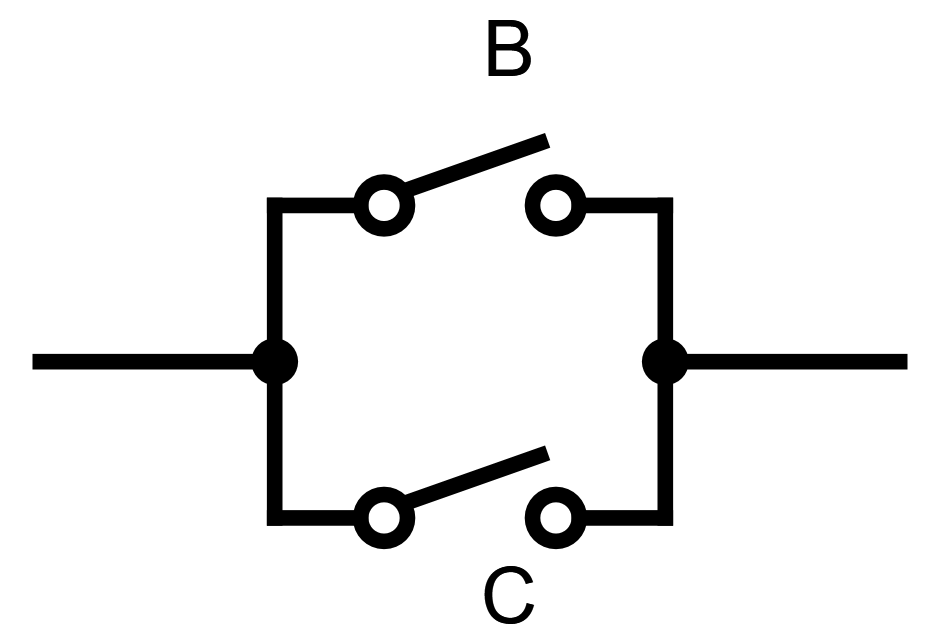
\includegraphics[width=.25\pagewidth]{p4-circuit}}

\end{document}